\newchapter{Perspective}{Perspective: Summary \& Discussion}{Perspective: Summary \& Discussion}
\label{chapter:5}

In this chapter we summarize the work presented in this dissertation.  We follow this summary with a discussion of the challenges that must be overcome if merging clusters are to reach their true potential as dark matter probes and discuss potential solutions to these challenges.

\section{Dissertation Summary}

Over the past century our understanding of the universe has under dramatic revisions which have culminated in once inconceivably accurate (percent level) measurements of the composition of the universe.
While the general scientific community agrees upon the composition of the universe, the properties of the bulk of this composition (dark matter and dark energy) are a mystery.
This dissertation has presented our recent efforts to better understand the properties of dark matter (DM).

In Chapter \ref{chapter:1} we provided a brief review of the history of DM (\S\ref{section:DMhistory}), showing that while Fritz Zwicky provided the first evidence of DM in 1933 \citep{Zwicky:1933ub} it wasn't until the work of Vera Rubin and collaborators \citep{Rubin:1970gu} in the 1970's that DM garnered much attention.
Three general candidates for DM originally dominated the debate.
One possibility was that it was simply massive compact objects made up of standard model particles, another was that it was some new particle, and another was the general relativity needed to be modified.
The MACHO experiment \citep{Alcock:2000bw} eventually ruled out the possibility that massive compact objects made up the bulk of DM, and merging galaxy clusters ruled out modified gravity \citep{Clowe:2006hr} and providing strong evidence for DM being a new particle.
We reviewed the generally accepted cold dark matter (CDM) properties (\S\ref{section:CDMproperties}) but provided motivation for considering that DM might actually interact with itself other than through gravity (SIDM model; \S\ref{section:SIDMmotivation}).
We reviewed the possible probes of SIDM (\S\ref{section:SIDMprobes}), highlighting  merging galaxy clusters {\S\ref{section:MergingClustersSIDMprobe}) and the four methods of constraining SIDM with observations of merging cluster.

In Chapter \ref{chapter:2} we introduced the the merging galaxy cluster DLSCL J0916.2+2951 (also known as the Musket Ball Cluster) and presented our multi-wavelength studies of the system.
Our photometric and spectroscopic observations show that the system consists of two subcluster separated by a projected distance of XXX and a redshift separation of XXX corresponding to a line-of-sight velocity difference of XXX.
Thus the two subclusters are close enough to be physically associated with one another.
Our weak lensing analysis of the two subclusters show that they have comparable mass XXX YYY, suggesting that they system is a major merger.
Our Sunyaev-Zel'dovich effect and X-ray observations show that the cluster gas is located between the two subclusters proving that the Musket Ball Cluster is a post merger system where the collisional gas has become dissociated from the effectively collisionless galaxies and DM.
Thus the Musket Ball Cluster is an excellent candidate to constrain the DM self-interaction cross-section ($\sigma_{\rm SIDM}$).

In Chapter \ref{chapter:3} we discussed the importance of understanding the dynamic history of mergers when attempting to use them to constrain the properties of DM.
We developed a new Monte Carlo based method to discern the properties of dissociative mergers and propagate the uncertainty of the measured cluster parameters in an accurate and Bayesian manner.
We verified it against an existing hydrodynamic N-body simulation, and applied it to two known dissociative mergers: 1ES 0657-558 (Bullet Cluster) and the Musket Ball Cluster.
We find that the dynamic properties of the Musket Ball represents a significantly different volume of merger phase space than the Bullet Cluster.
The Musket Ball Cluster, being $3.4^{+3.8}_{-1.4}$ times further progressed than the Bullet Cluster, could potentially provide tighter constraints on $\sigma_{\rm DM}$ since the offset between galaxies and dark matter should initially increase with time post-merger for  $\sigma_{\rm DM}>0$.

In Chapter \ref{chapter:4} we compare the locations of the galaxies, gas, and DM in the Musket Ball Cluster to provide insight into the properties of DM.
We are able to constrain the central gas distribution's projected centroid to within 9'' (57\,kpc at $z$=0.53), see \S\ref{section:GasLocation}.
Using both the extensive spectroscopic and photometric redshifts we are able to constrain the galaxy centroid of the northern subcluster to within 5.3" (33\,kpc at $z$=0.53) and the galaxy centroid of the southern subcluster to within 3.3" (21\,kpc at $z$=0.53), see \S\ref{section:GalaxyLocation}.
And using our tomographic WL method applied to the HST measured shapes we are able to constrain the projected WL centroid of the northern subcluster to within 13'' (82\,kpc at $z$=0.53) and the WL centroid of the southern subcluster to within 11'' (69\,kpc at $z$=0.53), see \S\ref{section:WLLocation}.
Our measurement of a significant offset of the gas between the DM in each subcluster enabled us to achieve the constraint $\sigma_{\rm DM} m_{\rm DM}^{-1} \lesssim 7$\,cm$^2$\,g$^{-1}$.
Given the dependence on the surface mass density of this method it is not surprising that this constraint is less than that achieved with more massive mergers \citep{Markevitch:2004dl, Bradac:2008gw, Merten:2011gu}.
Finally in this chapter we investigate the galaxy-WL offset since if DM self-interacts then the effectively collisionless galaxies might be expected to lead the DM post-merger.
While we find that the galaxies appear to be leading the WL centroid in the southern subcluster by $\sim$20.5'' (129\,kpc at $z$=0.53), see \S\ref{section:GalaxyWLOffset}, this only provides $\sim$85\% confidence that $\sigma_{\rm DM}>0$.
Furthermore when we account for the observation that the galaxy centroid appears to trail the WL centroid in the northern subcluster by $\sim$7.4'' (47\,kpc at $z$=0.53), the confidence that $\sigma_{\rm DM}>0$ falls to $\sim$55\%.
While the SIDM scenario is slightly preferred over the CDM scenario it is not significantly so.
SIDM simulations of the Musket Ball Cluster are needed to turn these observations into quantitative constraints on $\sigma_{\rm DM}$.


\section{Discussion on the Path Forward}

There are a number of outstanding uncertainties/challenges that must be overcome before merging clusters are proven capable of obtaining the necessary SIDM constraints to either measure sigma or constrain it to the point of being astrophysically uninteresting.

\subsection{Intrinsic Scatter in the Location of Galaxies and DM/Lensing}

Perhaps the most notable challenge are the results from the recent theoretical studies of SIDM effects in merging clusters by \citet{Kahlhoefer:2013wp} (which were presented in the arXiv one week before the completion of this dissertation).
While there are a number of promising results from their study which support claims made previously in this dissertation (e.g.: they confirm the expectation that the galaxy-DM offset increases following the merger, and also confirm that for some models of DM common mergers such of the Musket Ball Cluster can have more constraining power than extreme mergers such as the Bullet Cluster), one result from their study casts doubt on the possible effectiveness of merging galaxy clusters to constrain SIDM.
In particular, they find that the typical galaxy-DM offset ranges between $\sim$5--15\,kpc for allowable ranges of $\sigma_{\rm DM}$.
This is much smaller than the galaxy and WL centroid uncertainties typically measured for galaxy clusters ($\sim$20--100\,kpc).
And since most mergers don't occur directly in the plane of the sky, the observable projected offset will be $\lesssim$5--15\,kpc, assuming the \citet{Kahlhoefer:2013wp} results are correct.
Even disregarding intrinsic scatter of the galaxy-DM location and systematic offset effects due to the dissociated gas and other subcluster mass it will take a large number of dissociative mergers to reach the $\sim$10\,kpc offset level.

Take for example the Musket Ball Cluster studied in this dissertation.
We find that we are able to constrain the galaxy centroid in each subcluster to $\sim\pm$25\,kpc and the WL centroid in each subcluster to $\sim\pm$70\,kpc.
This roughly translates to a centroid offset uncertainty of $\sigma_{\rm offset}\sim$80\,kpc (again for argument's sake disregarding other systematic offset errors).
Since the offset measurement is largely Poisson noise dominated (i.e. $\sigma_{\rm offset}\propto N^{-1/2}$), it will take roughly 14--128 dissociative mergers\footnote{Assuming that two centroid offset measurements can be made for each dissociative merger, since there are two subclusters per dissociative merger.} similar to the Musket Ball Cluster to achieve the necessary centroid accuracy of $\lesssim$5--15\,kpc.
While this example is highly simplified, and it is not clear how general or accurate the \citet{Kahlhoefer:2013wp} results are,  it does highlight the magnitude of this challenge and the importance of investigating it further.

Along these lines, the intrinsic scatter between the location of the galaxies and DM in galaxy clusters is still not accurately known.
If the intrinsic scatter is of order the centroid measurement uncertainty then this will add significantly to the challenge of constraining SIDM with the galaxy-WL offset measurement in dissociative mergers.
Two immediate means of quantifying this intrinsic scatter is through studies of the scatter in existing simulations and observations of relaxed cluster systems.
A number of high resolution simulations of relaxed clusters exist \citep[e.g.][, which include both CDM and SIDM simulation]{Peter:2012vi, Rocha:2012tr}.
By treating the subhalos in the cluster simulation as galaxies, one could estimate the intrinsic galaxy-DM offset.
Alternatively a purely observational approach could study the galaxy-lensing offset in a sample of well measured relaxed clusters.
For example the Cluster Lensing and Supernova Survey with Hubble (CLASH) galaxy cluster sample (20 relaxed clusters, $\sim$5--30\,M$_\sun$) provides excellent weak and strong lensing data to locate the DM as well as 16-band photometric redshifts to identify cluster members for the galaxy population location.
Researchers of the Merging Cluster Collaboration are pursuing both avenues.

\subsection{Find and study more dissociative mergers}

Regardless of the magnitudes involved in the intrinsic scatter of the galaxy-WL/DM offset, it will be important to study as many dissociative mergers s possible in order to reduce this noise.
Fortunately the number of confirmed dissociative mergers has been increasing at a rapid rate (see Figure \ref{figure:N_Mergers}).
Prior to 2013 all of the dissociative mergers were serendipitously discovered, often requiring photometric, spectroscopic, lensing and X-ray observations for identification.
The rapid rise in the number of confirmed mergers after 2013 is due to the radio relic selection method.
Radio selection is an efficient way to select merging systems because the shock produced by a merger results in a ``radio relic'' (uniquely diffuse emission in an arc around part of the cluster, e.g. van Weeren et al. 2010).
So rather than needing photometric, spectroscopic, lensing and X-ray observations it is possible to identify dissociative mergers with just radio observations.
Thus wide-area radio surveys can provide many candidates. 
NVSS has already found a few dozen, and LOFAR is projected to find about 1000 \citep{Nuza:2012fu}.
The Merging Cluster Collaboration has begun an extensive follow-up of these radio relic mergers (see the red points in Figure \ref{figure:N_Mergers} after 2013) with Keck spectroscopy, Subaru and HST imaging, and Chandra and XMM X-ray imaging.

\begin{figure}
\centering
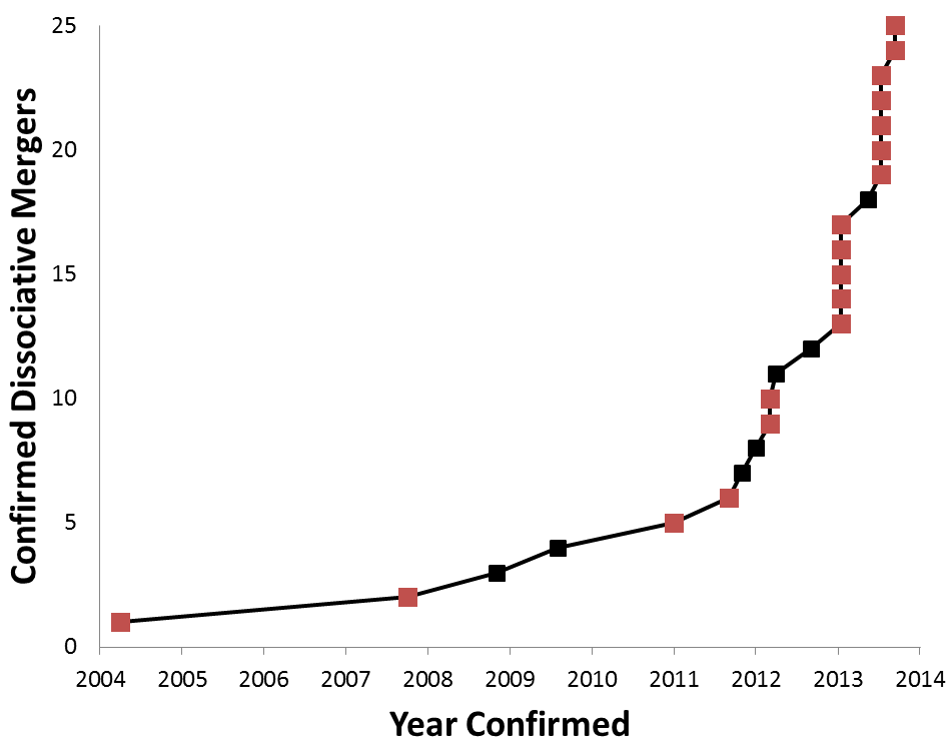
\includegraphics[width=4in]{Chapter5/NumberOfConfirmedDissociativeMergers.png}
\caption[Number of confirmed dissociative mergers as a function of time.]{
Number of confirmed dissociative mergers as a function of time.
The red points identify mergers that the Merging Cluster Collaboration are studying to  constrain the properties SIDM.
Up until 2013 dissociative mergers were all serendipitous discoveries.
The rapid rise in the number of confirmed mergers after 2013 is due to the radio relic selection method.
}
\label{figure:N_Mergers}
\end{figure}

Another promising avenue of dissociative merger discovery is with the optical-Sunyaev Zel'dovich effect identification method that lead to the discovery of the Musket Ball Cluster.
Since the DES optical survey \citep{Collaboration:2005vv} will overlap much of the SPT \citep{Ruhl:2004io} and ACT \citep{Hincks:2010ff} Sunyaev-Zel'dovich effect (SZE) surveys it will be possible to search for significant offset of an SZE peak between a bimodal distribution of galaxies.
Based on the simulated and observed SZ cluster counts in the SPT survey (Vanderlinde et al. 2010 \& Song et al. 2012) and the fraction of all clusters that are dissociative mergers (Forero-Romero et al. 2010) we estimate that $\sim$50 detectable dissociative mergers will be observed in the 4000 deg2 SPT-DES survey.  Selection bias will result in mergers with large mass (i.e. better signal-to-noise) and large projected separations (i.e. later stage mergers where the expected DM-galaxy offset is maximized).  These will potentially be some of the best dissociative mergers with which to constrain $\sigma_{\rm DM}$ .

Looking further into the future, the LSST optical survey \citep{Tyson:2002hn} will cover a larger area than DES and go much deeper.
When it is coupled with upcoming all-sky X-ray surveys (e.g. eROSITA), that will enable much better angular resolution of the gas compared to SPT and ACT, there is the possibility to discover discover thousands of dissociative mergers.
Additionally, LSST with have multi-band photometric redshifts and excellent lensing quality data.
Thus it is conceivable that the field of dissociative merger science will enter an era where the statistical errors no longer dominate the measurements. 

\subsection{Going from Observations to Dark Matter Constraints}

Beyond the challenges associated with making the galaxy-DM offset measurement there remains the challenge of translating that measurement into a constraint on $\sigma_{\rm DM}$.
--measure projected offset need 3D offset
-- need expectations for a given merger for varying dark matter cross-sections

Firstly, we can measure the projected offset of the two but this needs to be translated into a three-dimensional offset, and secondly 
The two primary obsticals in this regard are that we can measure the projected offset between the two but what is 

-note lack of distinction in offset between models
- merger property uncertainties

What are the major challenges to making merging clusters the best probes of SIDM

- intrinsic scatter in the M/L ratio \citep{Sheldon:2009fr}
-- look for assymetries in the M/L ratio

- turning observed galaxy-WL locations into $\sigma_{\rm DM}$ constraints




\textit{Should look at some proposal text}

The SIDM simulations of observed mergers are one of the most important aspects of the MC2 plan.  Not only are they necessary to place the tightest constraints on $\sigma$DM  (e.g. Randall et al. 2008), but by applying the same measurement techniques to the simulations as the observed mergers they will enable us to marginalize over systematic errors.  

Beyond the computational challenges of simulating SIDM (which our group has recently mastered, Rocha et al. 2012 \& Peter et al. 2012), it is highly non-trivial to simulate an actual observed merger. This is due to the fundamentally limited information observations provide for a given merger (Dawson 2012b). Thus a single observed merger can conceivably be represented by a wide range of simulated merger scenarios. To address this issue I will implement an importance sampling method to identify likely realizations of the observed merger in cosmological N-body simulations (Figure 3), extract a representative sample of these mergers, and in collaboration with MC2 members resimulate these with SIDM physics (Dawson et al. in prep).  Because each simulated realization of the observed merger will have an associated likelihood, I will be able to use the resulting $\sigma$DM  constraints of each realization to create a posterior probability density function.  This work will result in the first quantitative estimate of the $\sigma$DM  constraint uncertainty. 

Use results of the SIDM simulations of multiple observed dissociative mergers to place the best measurement or tightest constraint possible on $\sigma$DM.  

Because I will have taken care to properly quantify the uncertainty of dark matter constraints from each of the dissociative mergers (see Project 1), I will be able to properly combine the weighted expectations of each merger’s $\sigma$DM  constraint to effectively beat down the Poisson noise of the centroid offset measurement.   It is only through a consistent and systematic approach (such as the proposed) that one can properly combine the constraints of individual mergers. 


%\bibliographystyle{apj}
%\bibliography{Chapter1/chapter1}{}



%% The References
%\bibliographystyle{thesis}
%\begin{singlespacing}
%  \bibliography{Chapter3/chapter3}
%\end{singlespacing}
